\ylDisplay{Kada} % Ülesande nimi
{Oleg Košik} % Autor
{lõppvoor} % Voor
{2006} % Aasta
{G 3} % Ülesande nr.
{5} % Raskustase
{
% Teema: Dünaamika
\ifStatement
Vaatame lihtsa kada ehk ragulka konstruktsiooni. Elastne kummipael tõmmatakse kahe fikseeritud otspunkti vahele, laskmiseks asetatakse kivi paela keskele, pael tõmmatakse koos kiviga pingule ja lastakse vabaks. Kivi lastakse lendu horisontaaltasandi suhtes nurga $\alpha = \SI{10}{\degree}$ all. Leidke, kui kaugele peab laskja tõmbama kivi, et tabada märki, mis asub kadast $L = \SI{25}{m}$ kaugusel ning sellega samal kõrgusel. Kui suurt jõudu peab ta selleks paelale rakendama? Kummipaela pikkus pingestamata olekus on $l = \SI{60}{cm}$, mis on ühtlasi ka paela kinnituspunktide vahekaugus. Pael lugeda kaalutuks ning jäikusteguriga $k = \SI{50}{N/m}$. Kivi mass on $m = \SI{20}{g}$. Õhutakistusega ei ole vaja arvestada. Raskusjõu mõju kivi kiirendamisel kadas pole vaja arvestada.
\fi


\ifHint
Ragulkas salvestunud potentsiaalne energia muundub täielikult kivi kineetiliseks energiaks. Kummipaelale rakendatav jõud on leitav kummipaela pinge projektsioonist kivi lennu sihilisele teljele.
\fi


\ifSolution
Olgu kivi kiirus lasu järel $v$. Kiiruse horisontaalsuunaline komponent on $v_x = v \cos \alpha$ ja vertikaalsuunaline komponent $v_y = v \sin \alpha$. Kivi lennuaeg on
\[
t = 2 \frac{v_y}{g} = 2 \frac{v\sin\alpha}{g}
\]
ja lennukaugus
\[
L=v_{x} t=\frac{2 v^{2} \sin \alpha \cos \alpha}{g}=\frac{v^{2} \sin 2 \alpha}{g}.
\]
Siit
\[
v^2 = \frac{gL}{\sin 2\alpha}.
\]

\begin{center}
	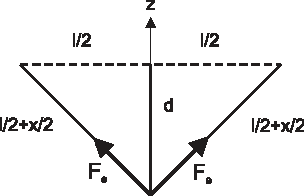
\includegraphics[width=0.5\linewidth]{2006-v3g-03-lah}
\end{center}

Kivi saavutab algkiiruse tänu kumminööri elastsele energiale. Kui nööri pikenemine võrreldes algolekuga on $x$, siis energia jäävuse seadusest saame
\[
\frac{k x^{2}}{2}=\frac{m v^{2}}{2},
\]
kust
\[
x^{2}=\frac{m v^{2}}{k} \quad\Rightarrow\quad x=\sqrt{\frac{m g L}{k \sin 2 \alpha}}=\SI{56,3}{cm}.
\]
Uurides ragulka geomeetriat näeme, et moodustuva täisnurkse kolmnurga hüpotenuus on $l/2+x/2$. Otsitav kaugus, millele tuleb nööri tõmmata, on seega
\[
d=\sqrt{(l / 2+x / 2)^{2}-(l / 2)^{2}}=\SI{49,8}{cm}.
\]
Kumminööris tekib elastsusjõud $F_e = kx$. Jõud, millega tuleb nööri tõmmata, võrdub selle jõu kahekordse projektsiooniga $z$-teljele:
\[
F=2 k x \frac{d}{l / 2+x/2} \approx \SI{50}{N}.
\]
\fi
}